\chapter{Results}    \label{results}
\section{Recruitment of Rvs to endocytic sites}

	\subparagraph{Curvature sensing or generation? }
	\mbox{}\\
Cellular membrane shape is a result of properties like rigidity, tension, intracellular pressure, and are influenced by the lipid composition and the proteins embedded in it1,2. Since tension, pressure, and rigidity all oppose membrane deformation, energy is required to deform and bend it. BAR domains can generate curvature if the energy required to deform the membrane is less than the energy spent in binding flat membrane.

\vspace{5mm}
			
Scaffolding as a curvature-generation mechanism has been extended to various types of BAR proteins, (Arkhipov et al., 2009; Frost et al., 2008; Henne et al., 2007; Itoh et al., 2005; Pykalainen et al., 2011; Saarikangas et al., 2009; Shimada et al., 2007; Yu and Schulten, 2013). In order for BAR scaffolds to impose membrane curvature, some requirement have to be met3: they have to have present a large membrane-interacting surface that can mediate membrane binding, have intrinsic curvature that can be imposed on the surface, and have a rigid structure that can overcome bending resistance of the membrane. Because of their shape (Peter 2004, Gallop 2006, Weissenhorn 2005), and their capacity to oligomerize into large assemblies on tubes (Mim 2012, Mizuno 2010, Takei 1999, Yin 2009), it has been suggested that BAR domains impose their shape on the membrane, and generate membrane curvature in cells. Further, tubulation both in-vivo and of liposomes is dependent on the rigidity of the central crescent-shaped domain4. The N-helix of NBAR domains can generate curvature independently of the BAR scaffold (Varkey 2010, Westphal and Chandra 2013).

\vspace{5mm}
For endophilin, the BAR domain is relatively far from the membrane, suggesting a mechanism dependent on the N-helix (Jao 2010). Different BAR domains thus likely employ different mechanisms to interact with the membrane for generating vesicles, and tubes (Ambroso 2014). For endophilin, for example, the N-helix is necessary for liposome binding5, while that of amphiphysin is important, but not necessary6. 

\vspace{5mm}
Curved BAR proteins that can induce curvature are also able to sense curvature: in-vitro, BAR domains show a preferential-binding to vesicles based on their intrinsic curvature. Curvature-generation and sensing seem to intrinsically couple mechanisms. That BAR domains are able to generate curvature does not imply that this is their function, at least in endocytocis: in-vivo, the significance of curvature-generation is not determined. Tracking over thirty different endocytic proteins in NIH-3TC cells (derived from mouse fibroblasts), TIRF imaging shows that Endophilin2 and Amphiphysin1 arrive late in the endocytic time-line right before scission7, suggesting they arrive when membrane tubes are already formed. 

\vspace{5mm}
In the case of Rvs, centroid tracking and averaging shows that the complex similarly localizes to sites late in the endocytic timeline, close to scission8. CLEM studies have further shown that Rvs localizes to sites after the membrane invaginations are about 60nm deep into the cytoplasm: Rvs localizes once membrane curvature is established. Whether this localization is dependent on membrane curvature, recognized by the BAR domain has not been shown. 

\vspace{5mm}
Rvs localization in yeast endocytosis
As has been shown before, Rvs localizes to endocytic patches at the yeast plasma membrane in the late scission-stage. When imaged at the plasma membrane, rather than a slow inward movement typical for coat proteins like Sla1, Rvs167-GFP shows a sharp jump into the cytoplasm, concomitant with scission8,9. The average lifetime of Rvs167-GFP is about 7secs, as measured by epifluorescence microscopy at the equatorial plane of a haploid yeast cell. 

\begin{figure}
\centering
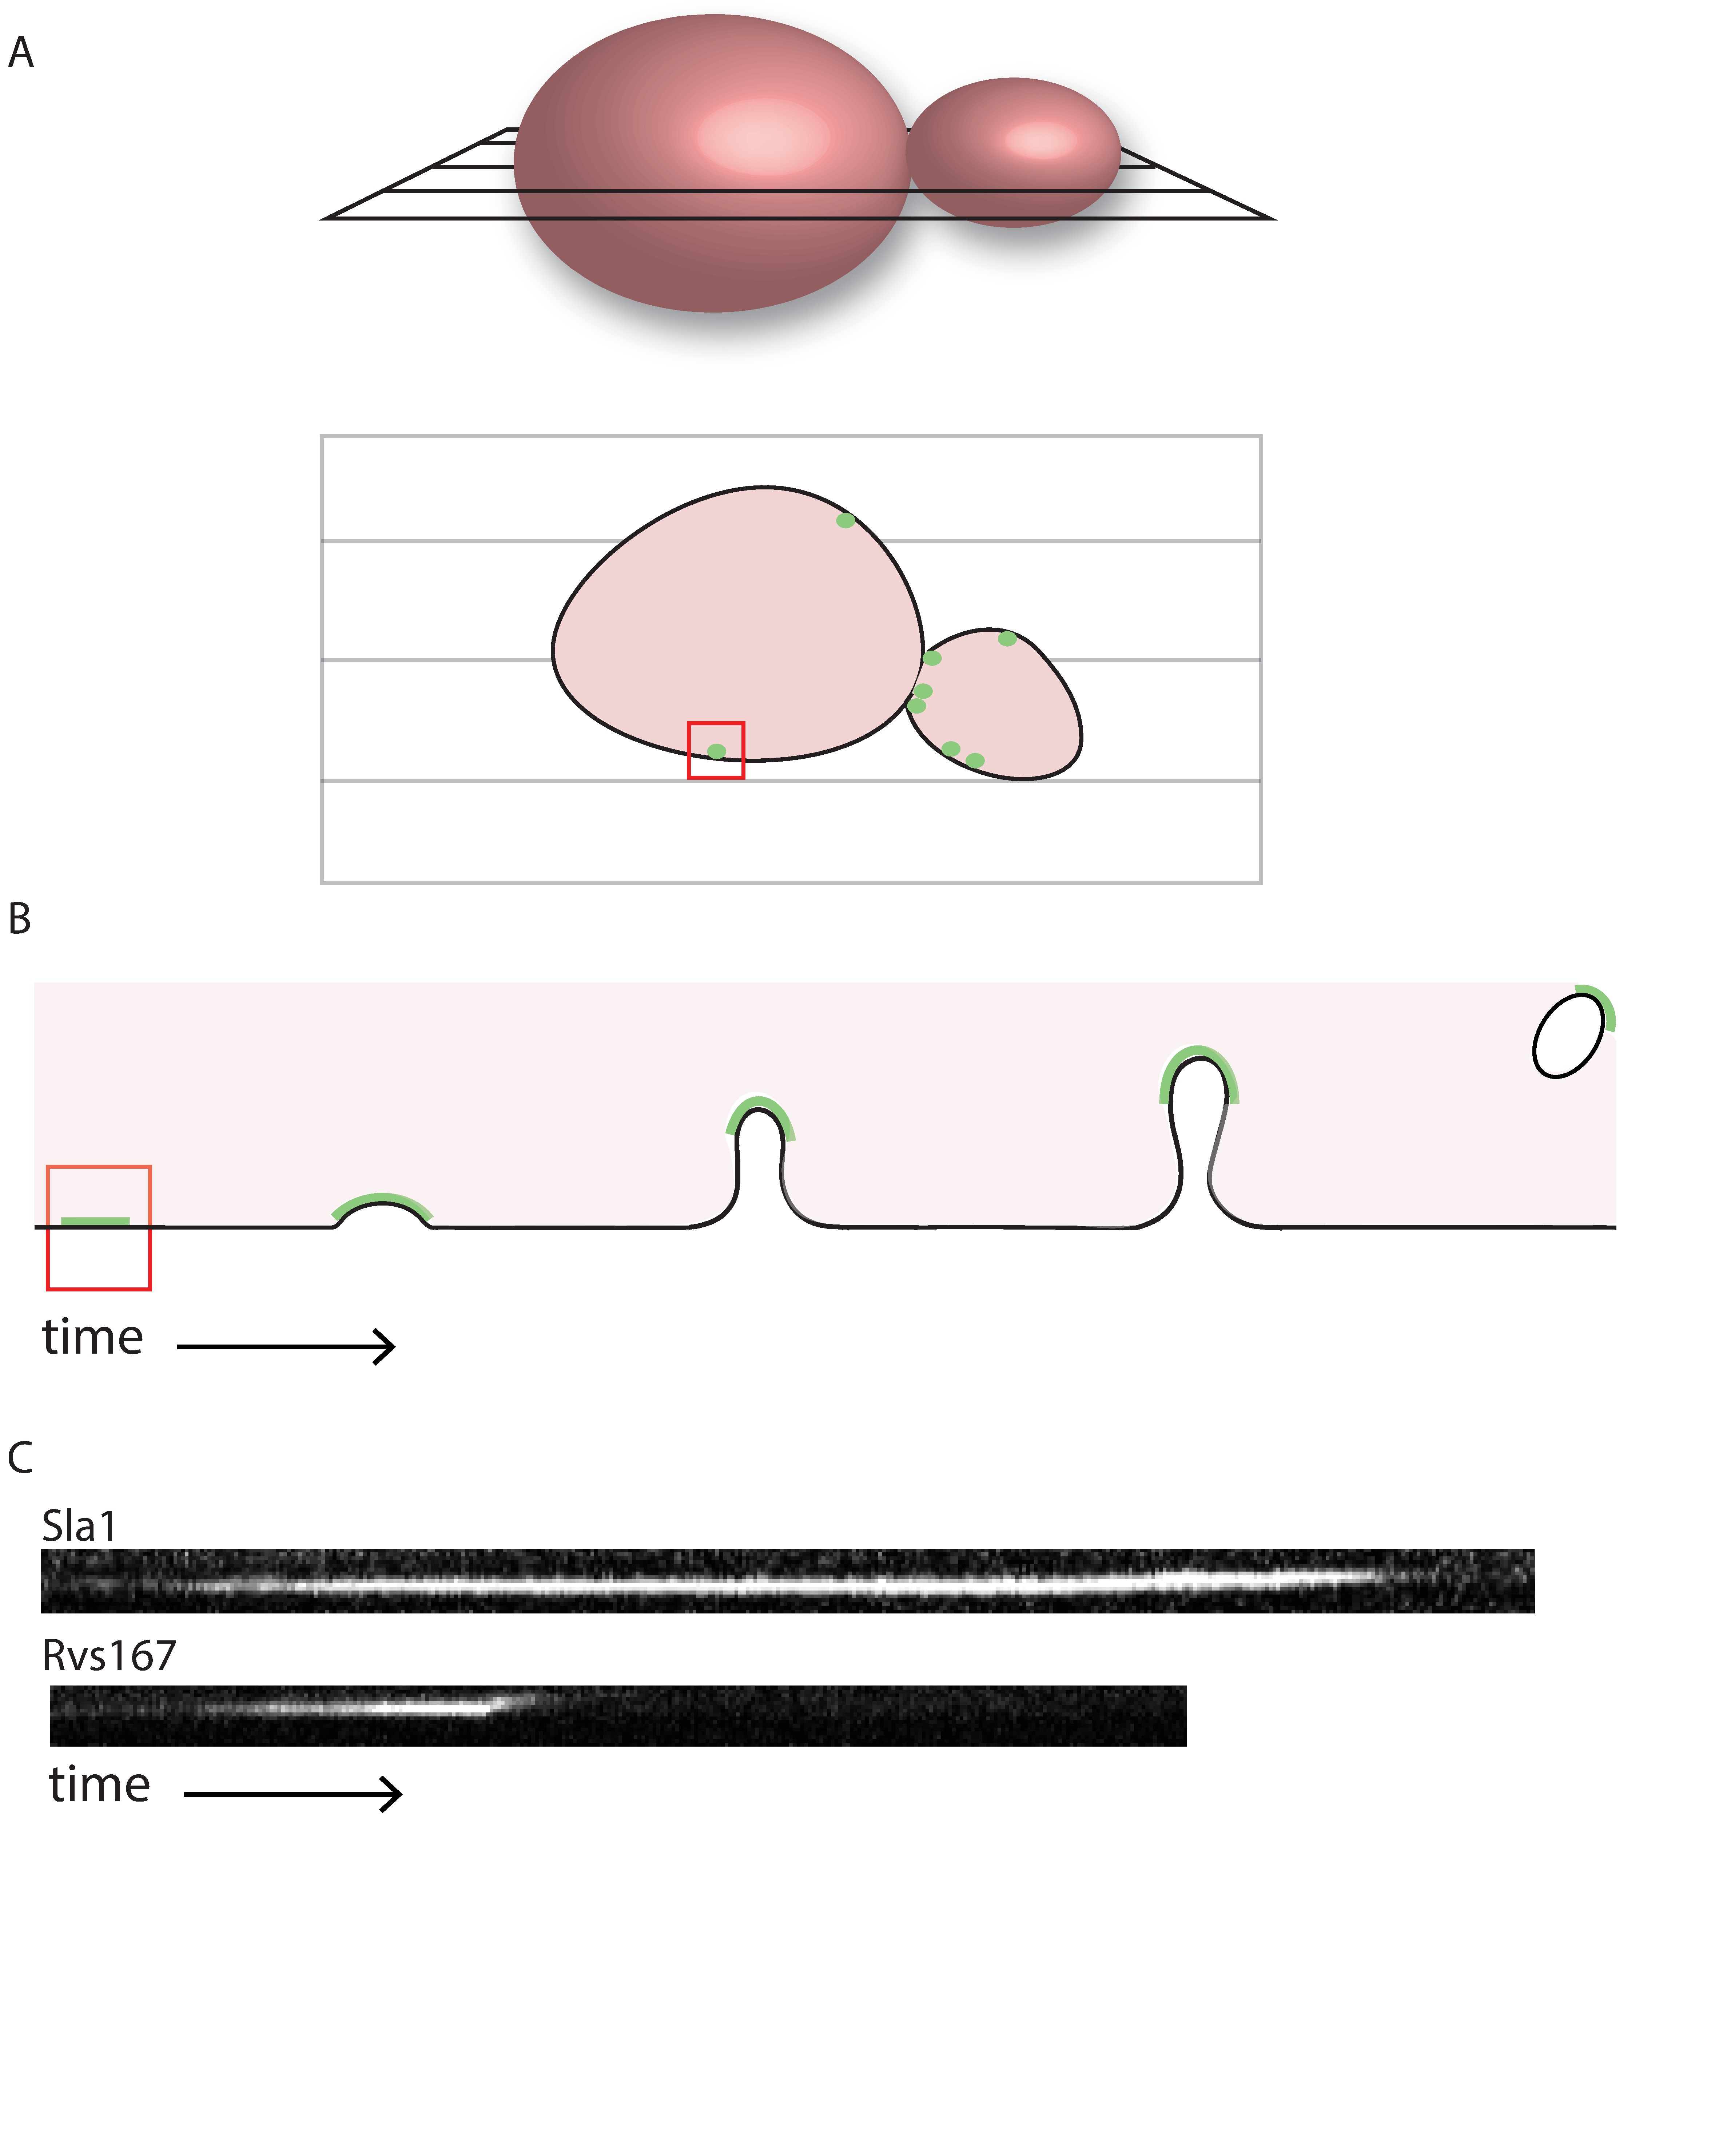
\includegraphics[width=10cm,height=10cm,keepaspectratio]{../../../figures/results_final/yeast_schemat_fig1_C}
%\includegraphics[width=10cm,height=10cm,keepaspectratio]
\caption{The Unit Circle \label{fig1_schematic}}
\end{figure}

	\subsection{BAR domain senses membrane curvature in-vivo}
	Rvs167 without the BAR domain, that is, Rvs167-delsh3 localizes to cortical patches (Fig.2.3). In order to test whether this localization is because of membrane curvature, I studied its dynamics in sla2del cells. Sla2 is a coat protein that acts as a linker between the membrane and the actin cytoskeleton, and allows forces generated within the actin network to be transmitted to the membrane10. In sla2del cells, rather than cortical actin patches, actin “flames” appear inside the cytoplasm. Electron microscopy shows that the membrane is flat in these cells: although actin is able to polymerize and recruit other actin-binding proteins, actin forces are decoupled from the membrane (Fig.2.2 schematic). 
	
	\vspace{5mm}
	In sla2del cells, Rvs167-GFP is recruited to the plasma membrane (Fig.2.3), while in sla2del cells expressing Rvs167-delsh3GFP (henceforth BAR-GFP), localization is removed, except for rare transient patches at the plasma membrane. 

	\subsection{SH3 domain is able to recruit Rvs in an
	actin-independent  	\\ manner}
	Full-length Rvs is able to localize to cortical patches in Sla2del cells. This localization must come from the SH3 domain, since BAR alone 	does not localize in these cells. We expected that the SH3 domain must interact with WASP or actin-binding proteins: an interaction with Abp1 has been shown, as well as with Las17, type I Myosins, and Vrp1. In order to prove this, I imaged BAR-GFP in cells treated with the actin sequestering agent LatrunculinA (LatA). LatA is a sea-sponge toxin that binds monomeric actin, and prevents incorporation of actin into filaments. Since a high actin turnover is required at endocytic sites, LatA effectively disassembles WASP components and other actin-binding proteins of the endocytic machinery, and blocks endocytosis. 

	\vspace{5mm}
	Surprisingly, full-length Rvs is localized to the plasma membrane in spite of the LatA treatment, suggesting that the SH3 domain is able to recruit Rvs to the plasma membrane. This recruitment occurs in the absence of a BAR-membrane interaction, since BAR-GFP localization is completely removed in LatA treated cells. Rvs167-GFP patches are transient, so an assembly-diassembly mechanism is mediated by the SH3 domain outside of its BAR domain interaction. Localization of Rvs161, which does not have an SH3 domain, is also removed by LatA treatment, supporting the conclusion that the BAR domain senses membrane curvature in-vivo. 

\begin{figure}
	\centering
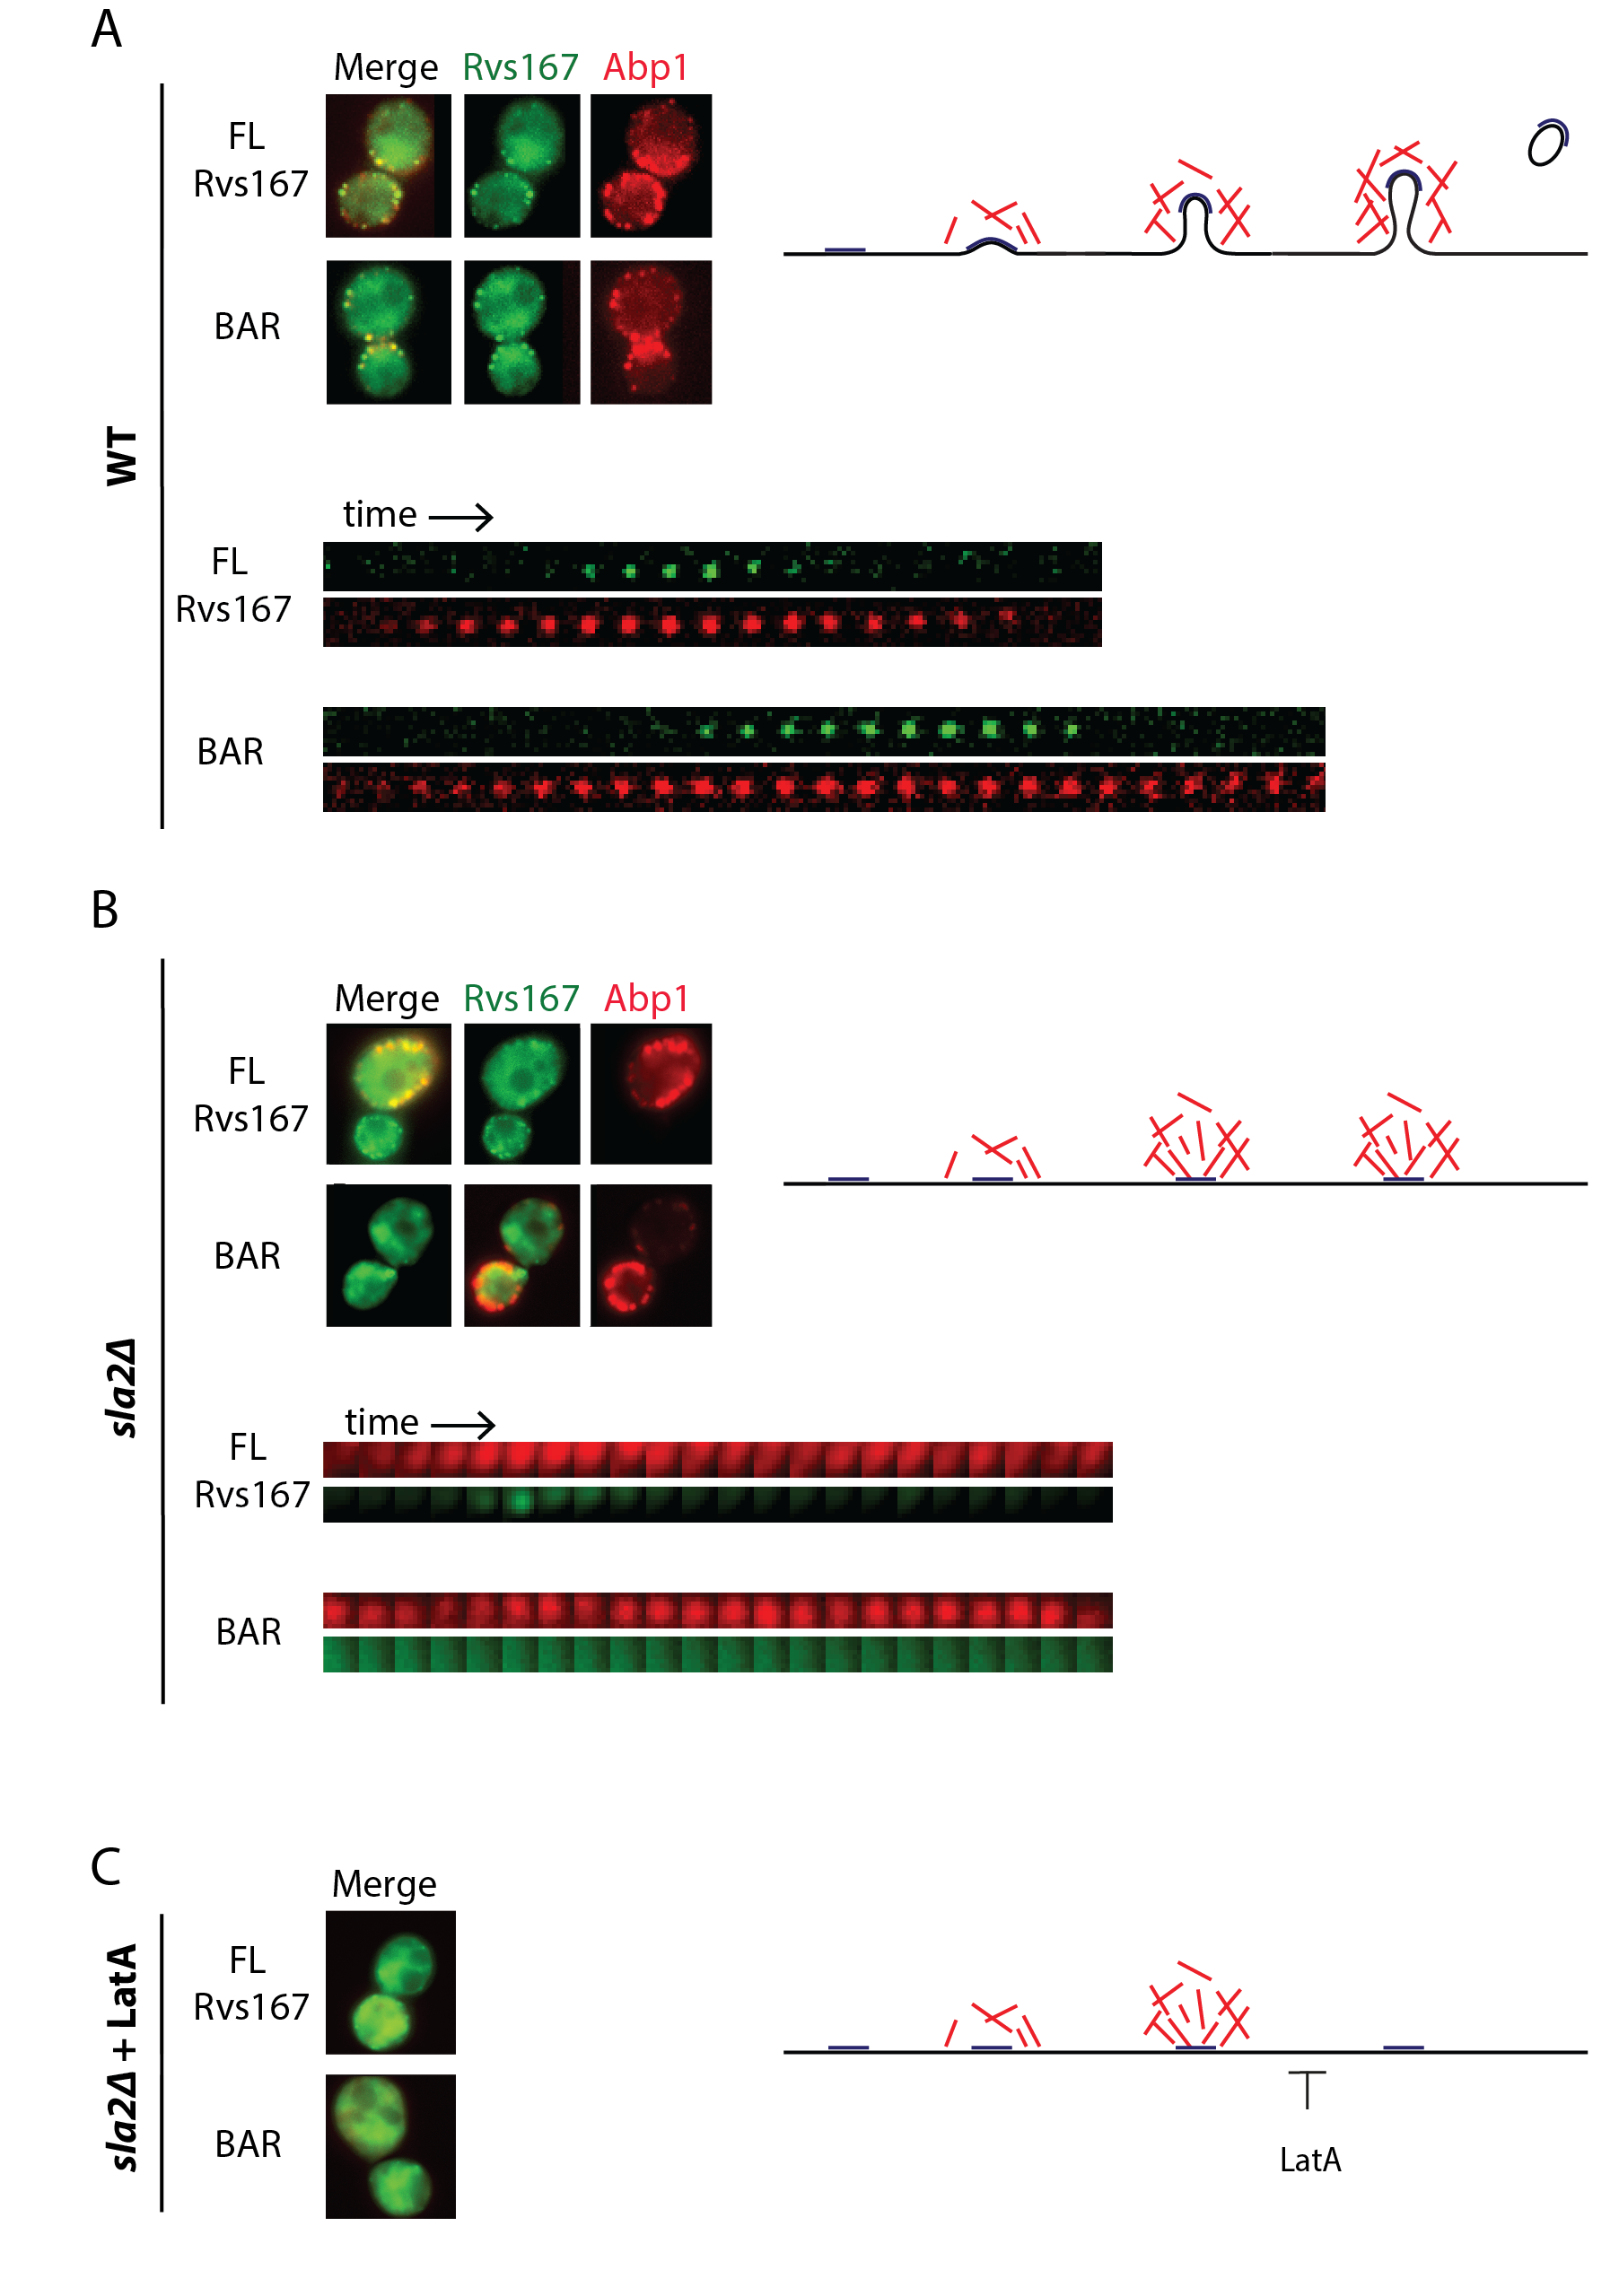
\includegraphics[width=22cm,height=22cm,keepaspectratio]{../../../figures/results_final/sla2_del_final3}
	\caption{Rvs localization in sla2 deletion\label{fig2_sla2del}}
\end{figure}

	\subsection{What does the SH3 domain interact with?}
		\subsubsection{Vrp1}
		\subsubsection{Type 1 myosins}
		\subsubsection{Las17}


	\subsection{Other potential mechanisms of assembly/ disassembly of Rvs}		
			\subsubsection{Interaction with Calmodulin}
			\subsubsection{FBAR protein Bzz1}
				
\section{Role of the SH3 domain}	
Is likely that SH3 domains, are involved in modulating oligomerization (5, 14) and MC-S, G (15, 82). 	
\section{Role of the N-helix}			
		
\section{Scission mechanisms}

	\subsection{Membrane scission is not dependent on Vps1}
	Yeast dynamin is the obvious solution to membrane scission. Although none of the three dynamin- like proteins has a proline-rich domain, one of the yeast dynamins, Vps1 has been suggested to be involved in endocytosis11,12. Rooij et al., suggest that Vps1 localizes to endocytic sites in the late scission stage, and that the vps1Δ rvs167Δ double mutant increases membrane retraction rates after invagination, an indication of scission failure. Vps1-GFP does not localize to endocytic sites in Gadila et at.,13, but localizes to the golgi body and to vacuoles. Kishimoto et al, do not find a colocalization between Vps1 and Abp1 localization, and also report that the vps1Δ rvs167Δ  double mutation does not affect membrane retraction rates. Vps1 tagged with both GFP as well as superfolded GFP, and imaged by TIRF microscopy fails to colocalize with Abp1 (data not shown, personal communication with Andrea Picco). The debate concerning the involvement of Vps1 in membrane scission in yeast has been compounded by the possibility that the GFP tag at the Vps1 C-terminal could interfere with its localization to endocytic sites, or its interaction with the Rvs complex. 
	
	\vspace{5mm}
	In order to exclude the possibility of interference from the GFP tag, I investigated the role of Vps1 by studying coat and scission proteins in vps1Δ cells. The late coat protein, Sla1 is used as a marker for coat movement, and Rvs167 marks scission time. Centroid tracking and averaging is performed as described in Picco et al., and inward movements of the both in wild-type and vps1Δ cells are compared. 

%	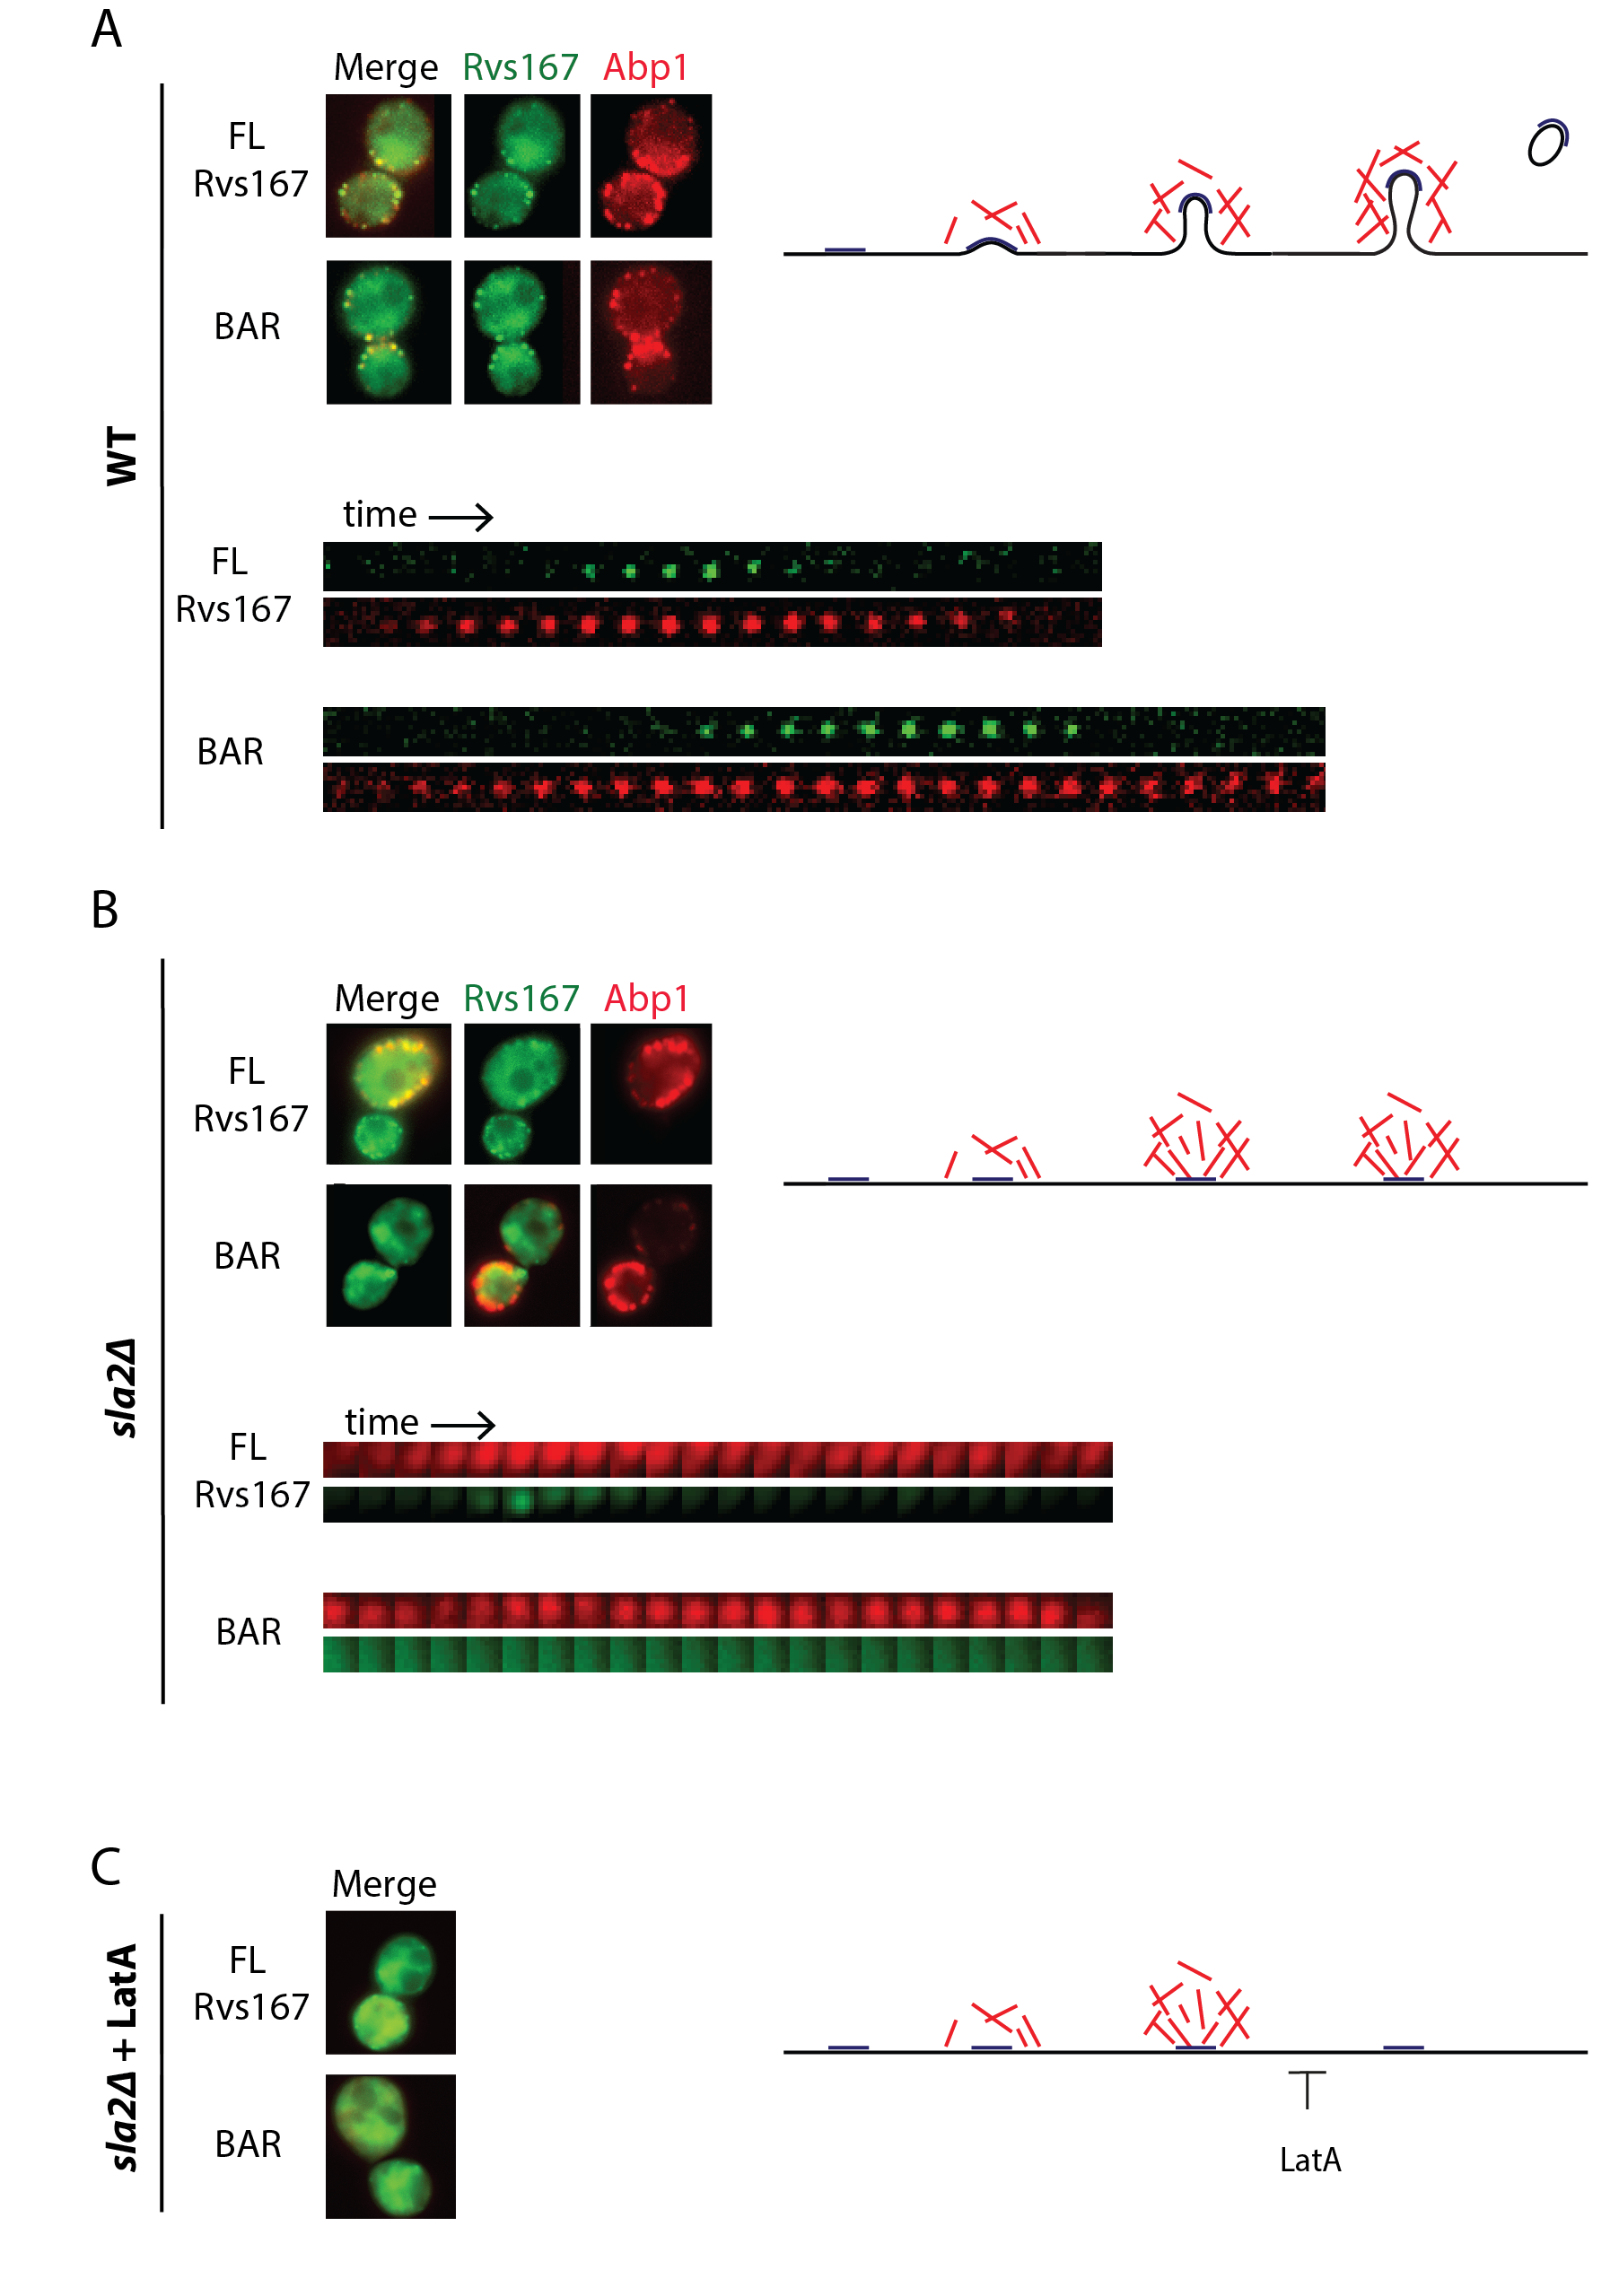
\includegraphics[width=20cm,height=20cm,keepaspectratio]{../../../figures/results_final/sla2_del_final3}
	\begin{figure}
	\centering
	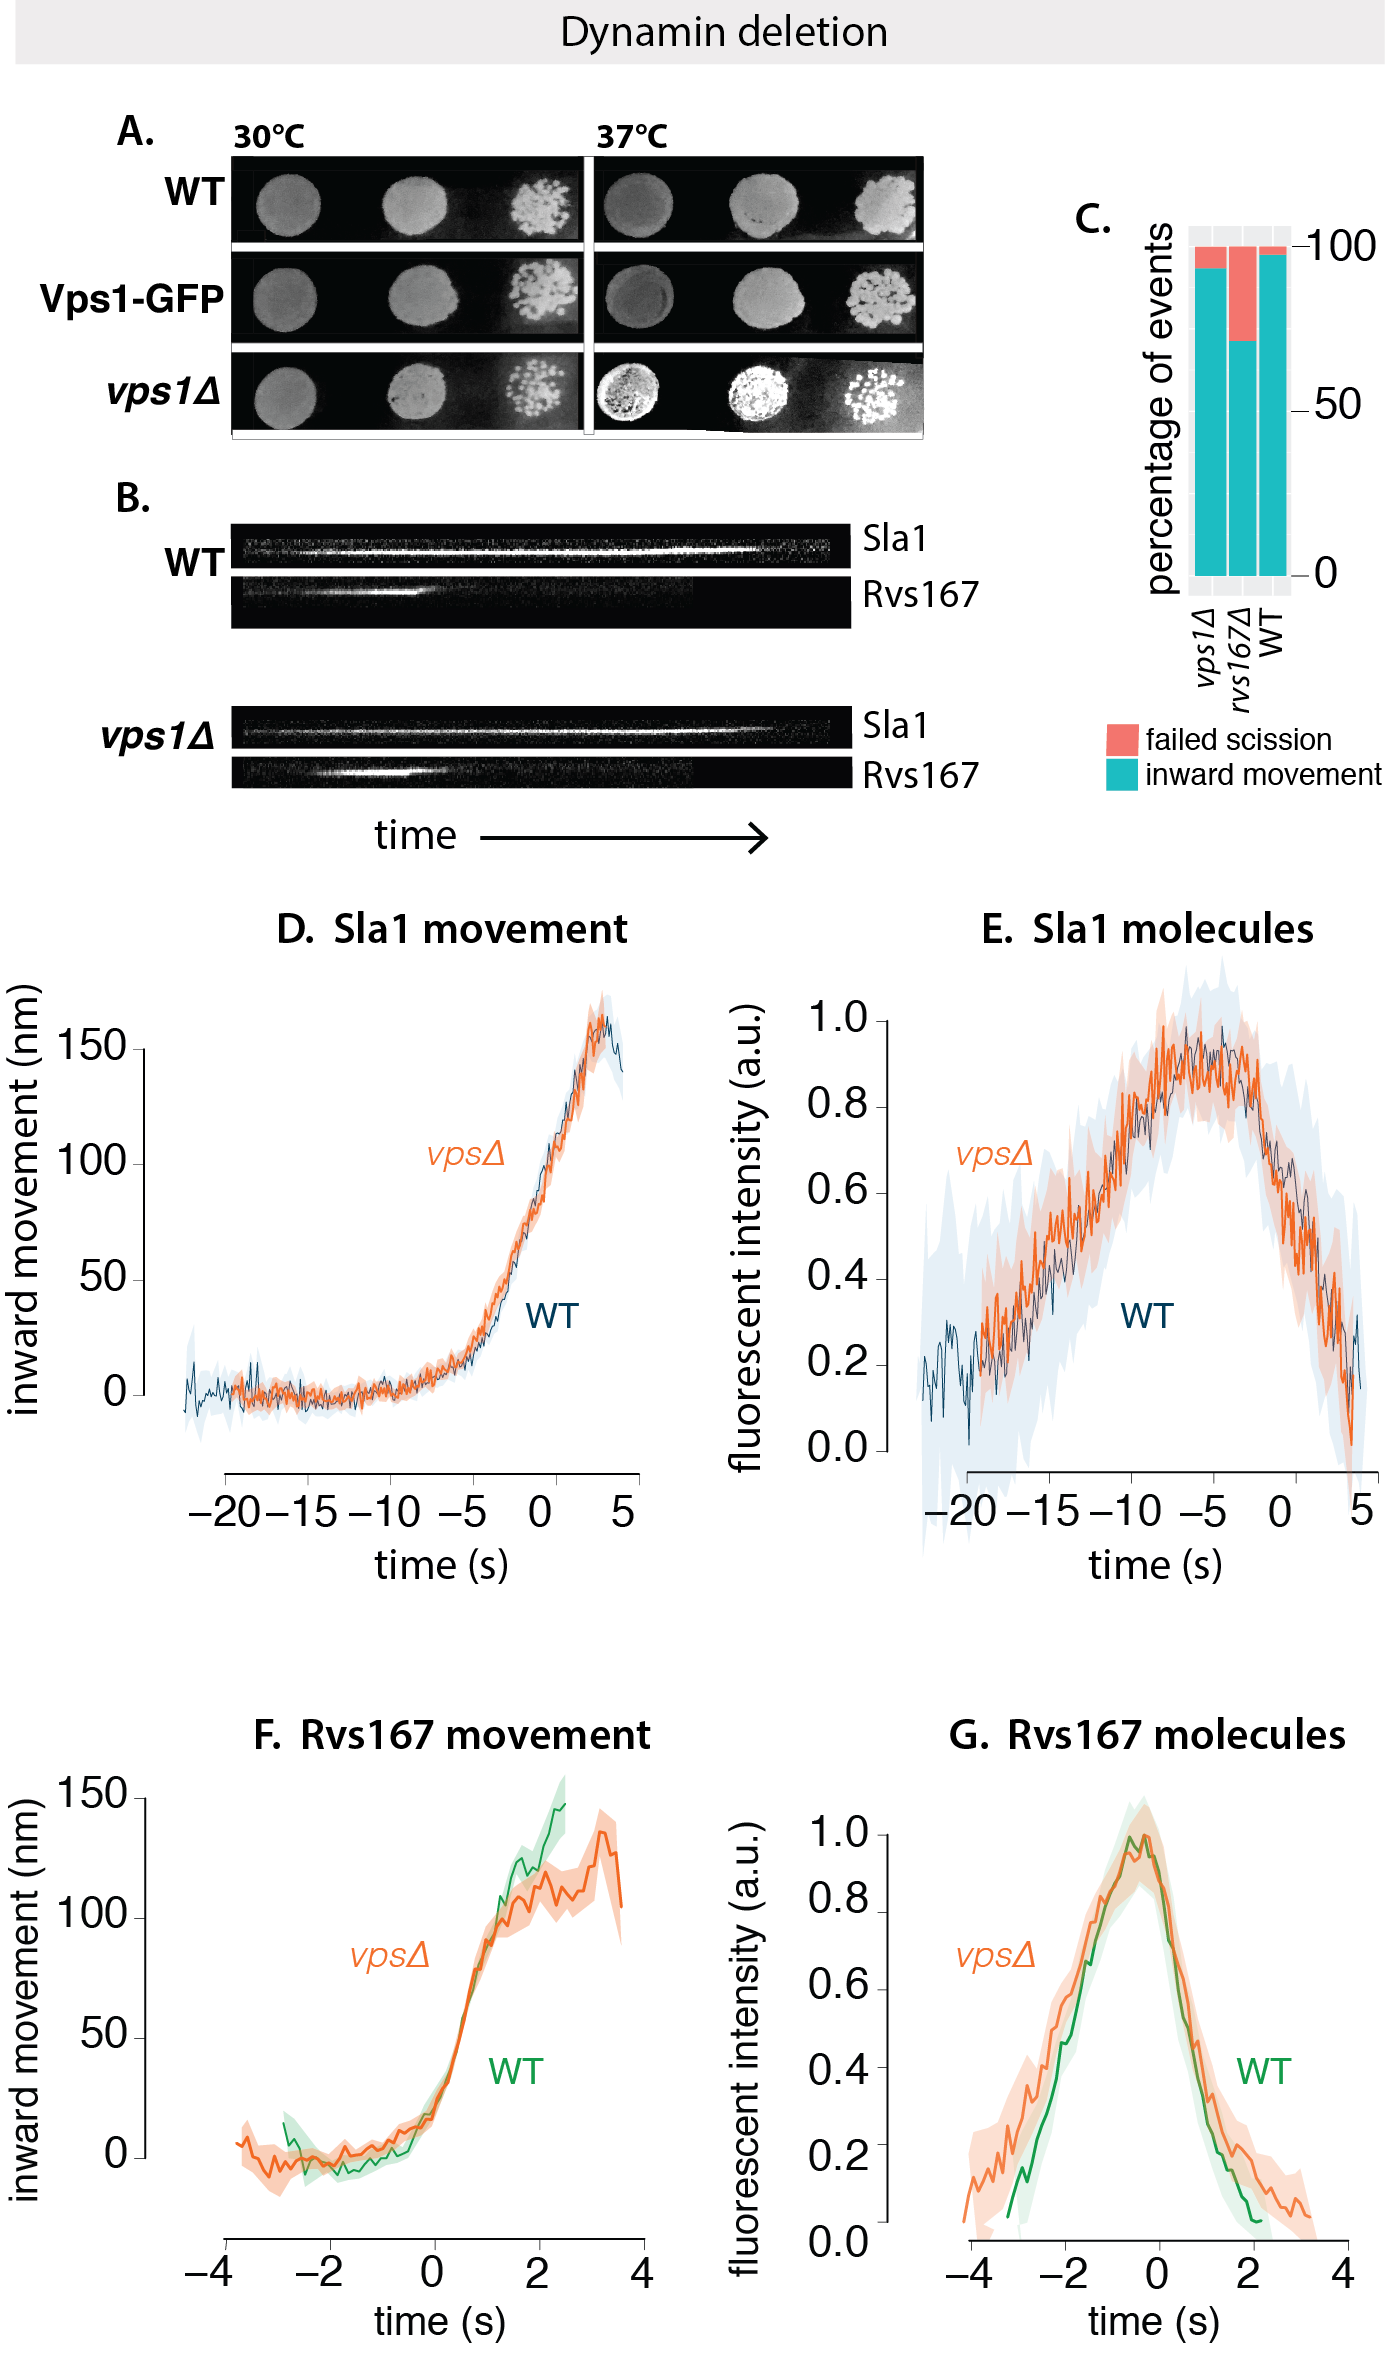
\includegraphics[width=23cm,height=23cm,keepaspectratio]{../../../figures/results_final/vps}
		\caption{Rvs localization in vps deletion\label{fig3_vpsdel}}
	\end{figure}

	
	\vspace{5mm}
	vps1Δ cells exhibit a growth defect at 37C, as has been reported11. Sla1-GFP accumulates at the plasma membrane, moves inwards, and disassembles like in WT. The average lifetime of Sla1-GFP at endocytic patches remains unchanged. In WT cells, Sla1 moves into the cytoplasm about 140nm before membrane scission occurs. If Vps1 was required for membrane scission, Sla1 would be expected to undergo delayed or failed scission. However, vps1Δ does not increase the rate of membrane retraction. Inward movement of Sla1 is also not changed: it moves inward at the same rate, and to similar maxima of 140nm. Further, the averaged centroid of Rvs167 would not show the sharp jump into the cytoplasm if scission failed. If scission was delayed, the average lifetime of Rvs167 would increase. The inward movement of Rvs167, and its average lifetime, however, remains the same as in WT. I conclude that if Vps1 does localize to endocytic patches in S.cerevisiae, it is not involved in regulating membrane scission.  


	\subsection{Lipid hydrolysis and membrane scission}
	
	\subparagraph{Can lipid hydrolysis drive membrane scission?}
	Another hypothesis has proposed that regulated lipid hydrolysis can cause vesicle scission19. Phosphatidylinositols (PIs) and their derivatives play important roles in many cellular processes including membrane trafficking and cell signalling. Conversion between lipid types is driven by kinases, lipases, and phosphatases and controlled throughout the membrane trafficking pathway. 
	
	\vspace{5mm}
	Phosphatidylinositol(4,5)-biphosphate (PI (4,5) P2) is an important lipid type found at the cell surface, and is enriched and depleted from endocytic sites at the plasma membrane in concert with the assembly and disassembly of the endocytic machinery. Synaptojanins form a subset of inositol polyphosphate 5-phosphatases that hydrolyze PI(4,5)P2 to PI(4)P by removing the phosphate at the 5’ position of the inositol ring, and play a role in CME and intracellular signalling, as well as in modulating the actin cytoskeleton14. Synaptojanins localize to endocytic sites, and in mammalian cells, disruption of Synaptojanin genes results in cellular accumulation of PI(4,5)P2 and coated vesicles at the plasma membrane, suggesting a role for lipid hydrolysis in releasing coat proteins from nascent vesicles. Syaptojanins contain an N-terminal homology domain with the cytoplasmic domain of the yeast SAC1 gene, that is implicated in lipid metabolism, actin morphology, and vesicle transport in the secretary pathway15. A central catalytic domain is followed by a proline-rich C-terminal regions that are the canonical interaction partners of SH3 domains: they are known to interact with actin binding proteins and BAR domain proteins, potentiating also a role in membrane invagination and scission. 
		
	\vspace{5mm}
	The yeast encodes three Synaptojanin-like proteins- Inp51, Inp52 and Inp53- that regulate phospholipid metabolism. Double deletion of Inp51 and Inp52 has been shown to increase the lifetime of endocytic proteins and produce aberrant membrane invaginations that could indicate scission failure and defective endocytosis, although uptake of extracellular membrane appears to proceed in spite of the morphological aberrations16,17. Deletion of Inp52 along with Rvs167 increases scission failure rate, supporting a possible role in membrane scission18. Loss of inp51 mutation shows a increase in bulk PIP2 level, although chages in PIP2 levels have not been reported for mutations of inp52, and are not measured locally at the endocytic sites19,20.

	\subparagraph{Loss of yeast synaptojanins does not significantly affect coat and Rvs dynamics}
	\mbox{}\\
	In a model proposed by Liu et al, Synpatojanins and BAR proteins interact to regulate PI(4,5)P2 hydrolysis, which in turn drives membrane scission. Here, the Rvs scaffold on the membrane tube protects the underlying PIP2 from hydrolysis. Synaptojanin arrives at sites, and hydrolyses unprotected PIP2. This generates a boundary between BAR-protected PIP2 at the tube and PIP at the bud tip. The lipid boundary produces a line tension at the interphase that would generate enough force to pinch off a vesicle. 
		
	I tested this model by investigating the effect of synaptojanin deletion on coat and scission proteins. First, of the three yeast Synaptojanins, only Inp52-GFP localizes to cortical patches. Dual-color imaging and time alignment with Abp1 as described in Picco et al., shows that Inp52 localizes to endocytic sites at the late stage of scission along with Rvs. The centroid of Inp52-GFP can be localized to the tip of the invaginated tube, consistent with the Liu theory of membrane scission: spatial and temporal localization is consistent with influence on scission. Inp51-GFP exhibits a diffuse cytoplasmic signal, while Inp53 localizes to patches within the cytoplasm, likely to the trans-golgi network, as has been noted in other work. 

	\begin{figure}
	\centering
	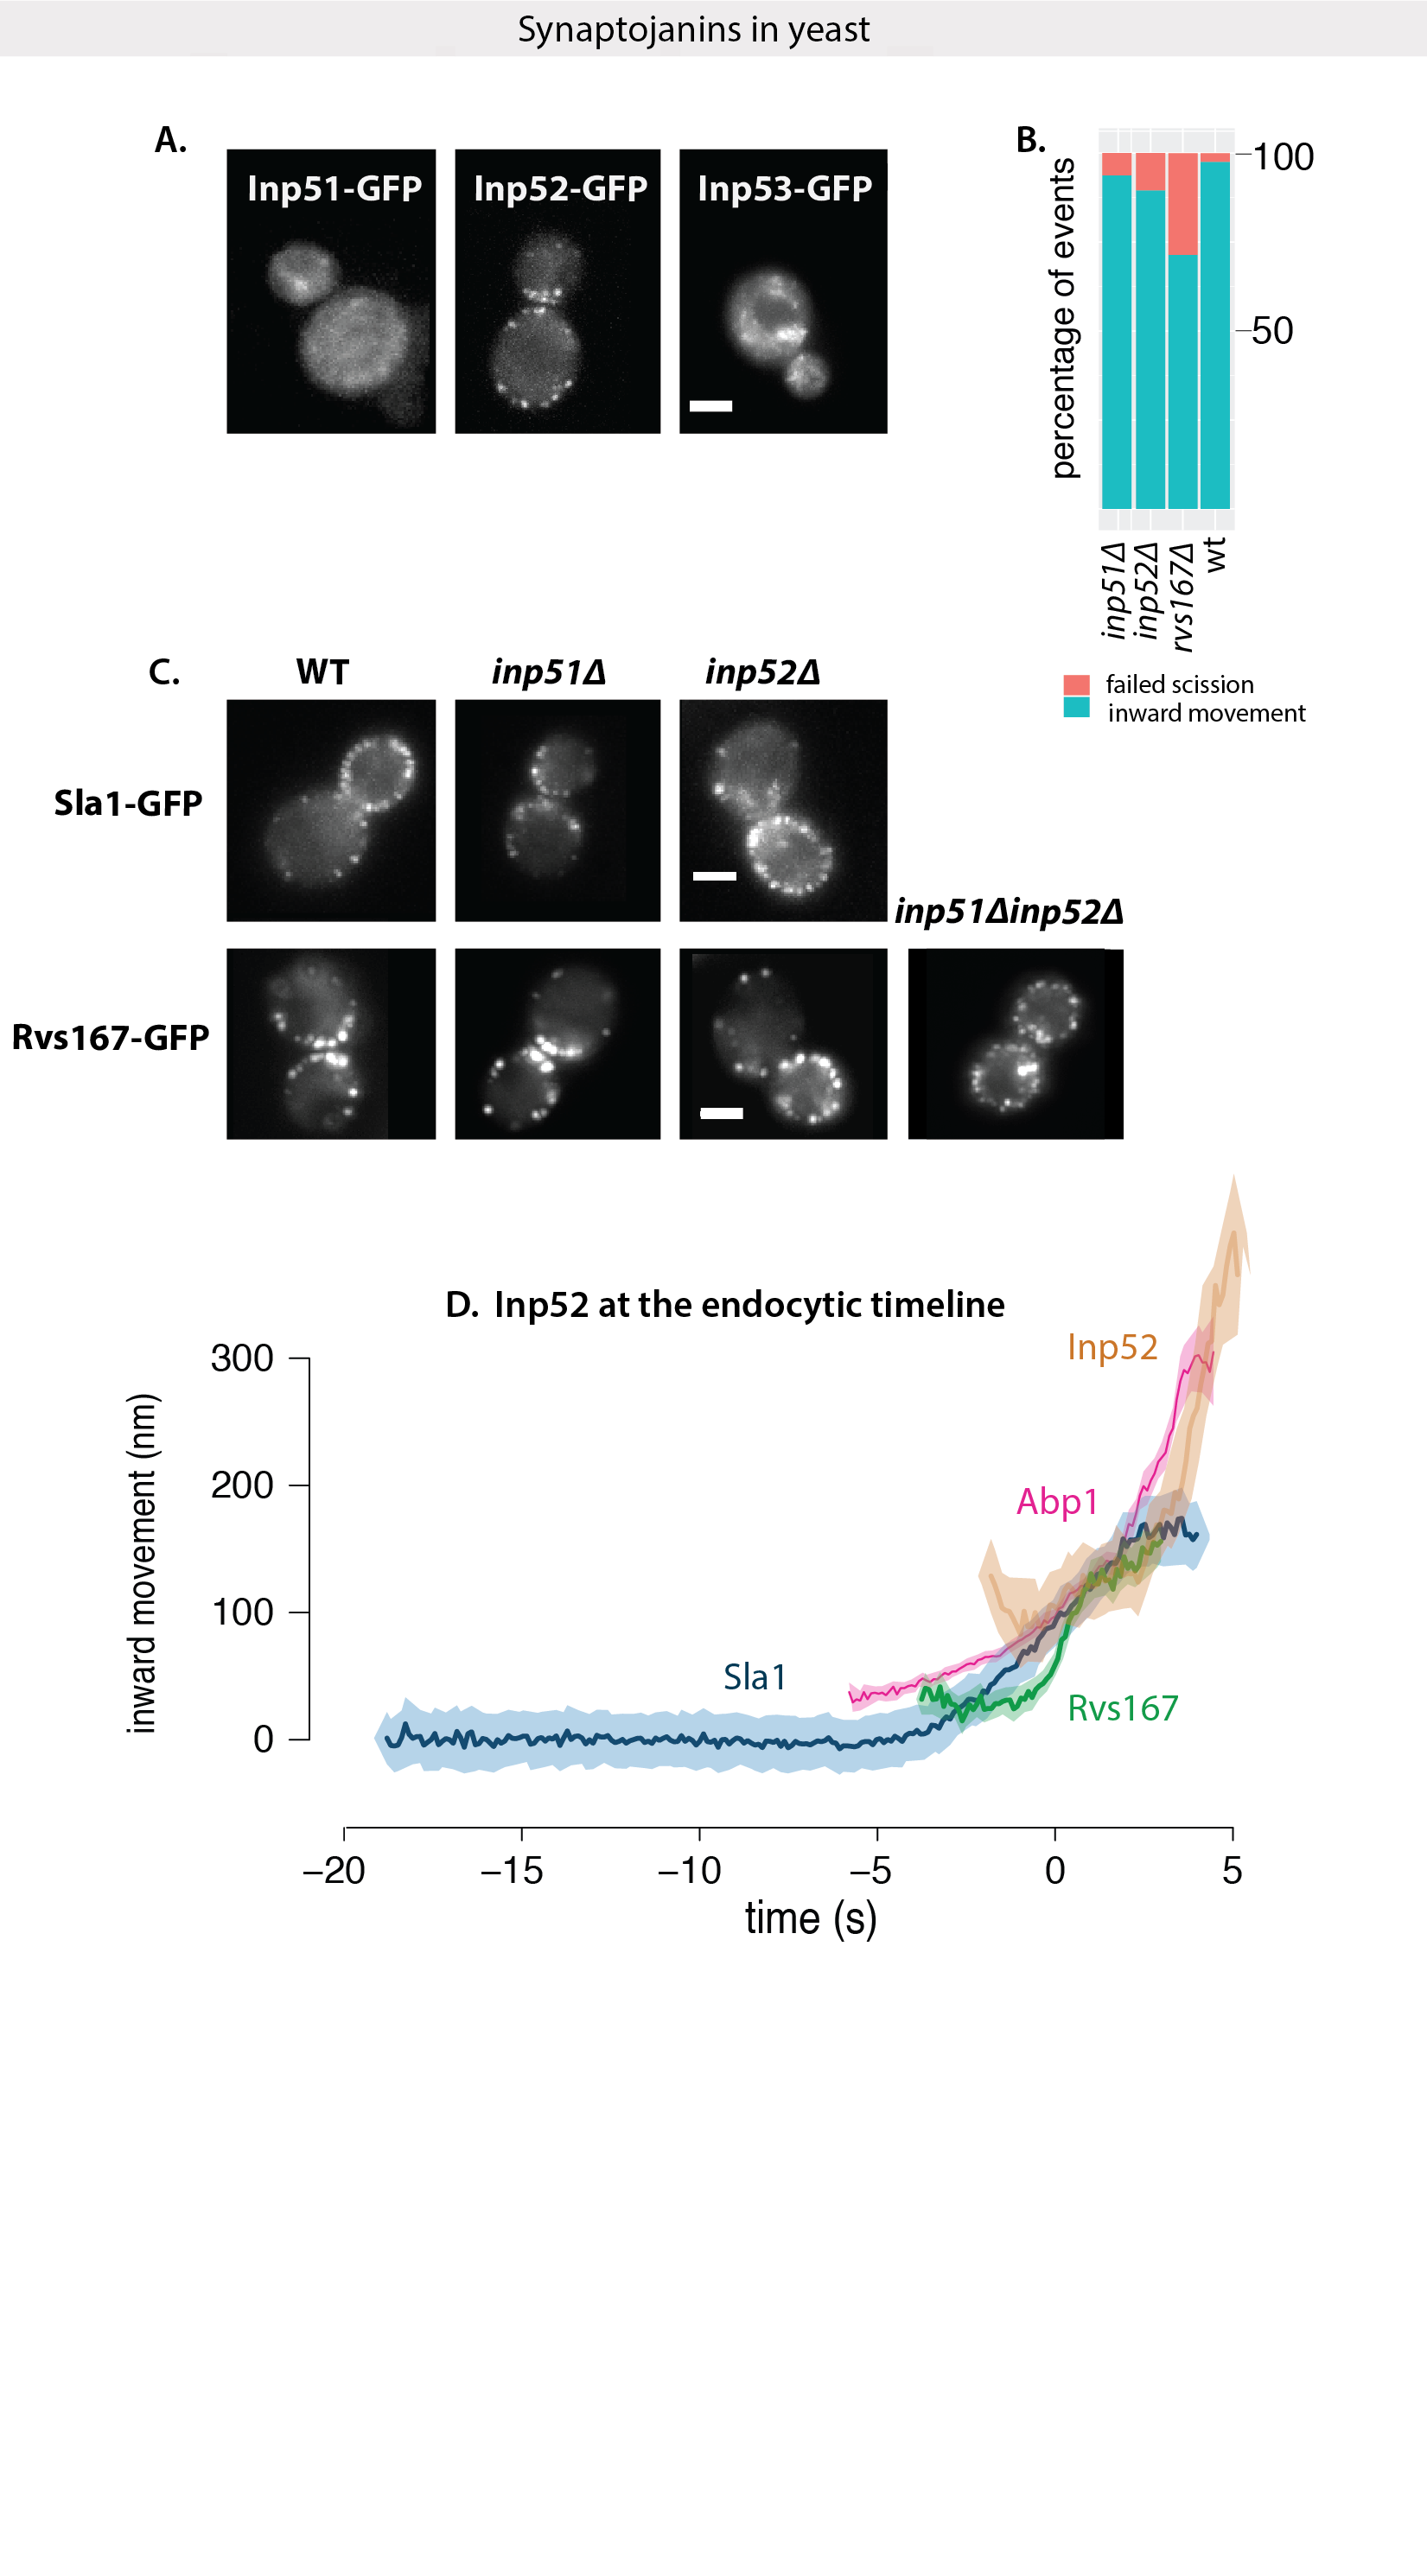
\includegraphics[width=20cm,height=20cm,keepaspectratio]{../../../figures/results_final/inp}
	\caption{Yeast synaptojanins \label{fig4_inp}}
	\end{figure}

	\vspace{5mm}
	Deletion of Inp52 does not affect the speed of membrane invagination, as reported by the movement of the Sla1 centroid. Sla1-GFP patches are assembled and disassembled, as are Rvs167-GFP patches. All Sla1-GFP patches in the movies analysed (n=13 cells) move inwards.  Dense clusters at bud neck are not considered. 72.9\% of Rvs167-GFP patches move inwards into the cytoplasm (n=4 cells, 37patches). Remaining patches are disassembled without apparent inward movement. Dense clusters at bud neck are not included in the statistics. Vesicle scission appears to occur similar to wild-type, since the Rvs167 centroid moves inwards to approximately the same distance into the cytoplasm, indicating that the base of the vesicles are likely at the same position as in wild-type. Both Sla1 and Rvs167 centroids however, persist post-scission (arrowheads in figure) instead of disassembling immediately like in the WT. Since majority of the patches move inwards, and the increase in the lifetime of Rvs is post-scission, I find that the data is consistent with a role for Inp52 in vesicle uncoating, rather than a primary role in membrane scission, with the aberrations in plasma membrane morphology consequent of failure to recycle components, rather than scission. 

	\vspace{5mm}
	Deletion of Inp51 does not affect Rvs167 or Sla1 centroid movement. All Sla1-GFP patches move inward (n=19 cells). 93\% of Rvs167-GFP patches move inward (n=3 cells, 44 patches), similar to WT. Assembly of Rvs167 in the Inp51del is slowed, the implication of this delay is not thus far clear. 

	\begin{figure}
	\centering
	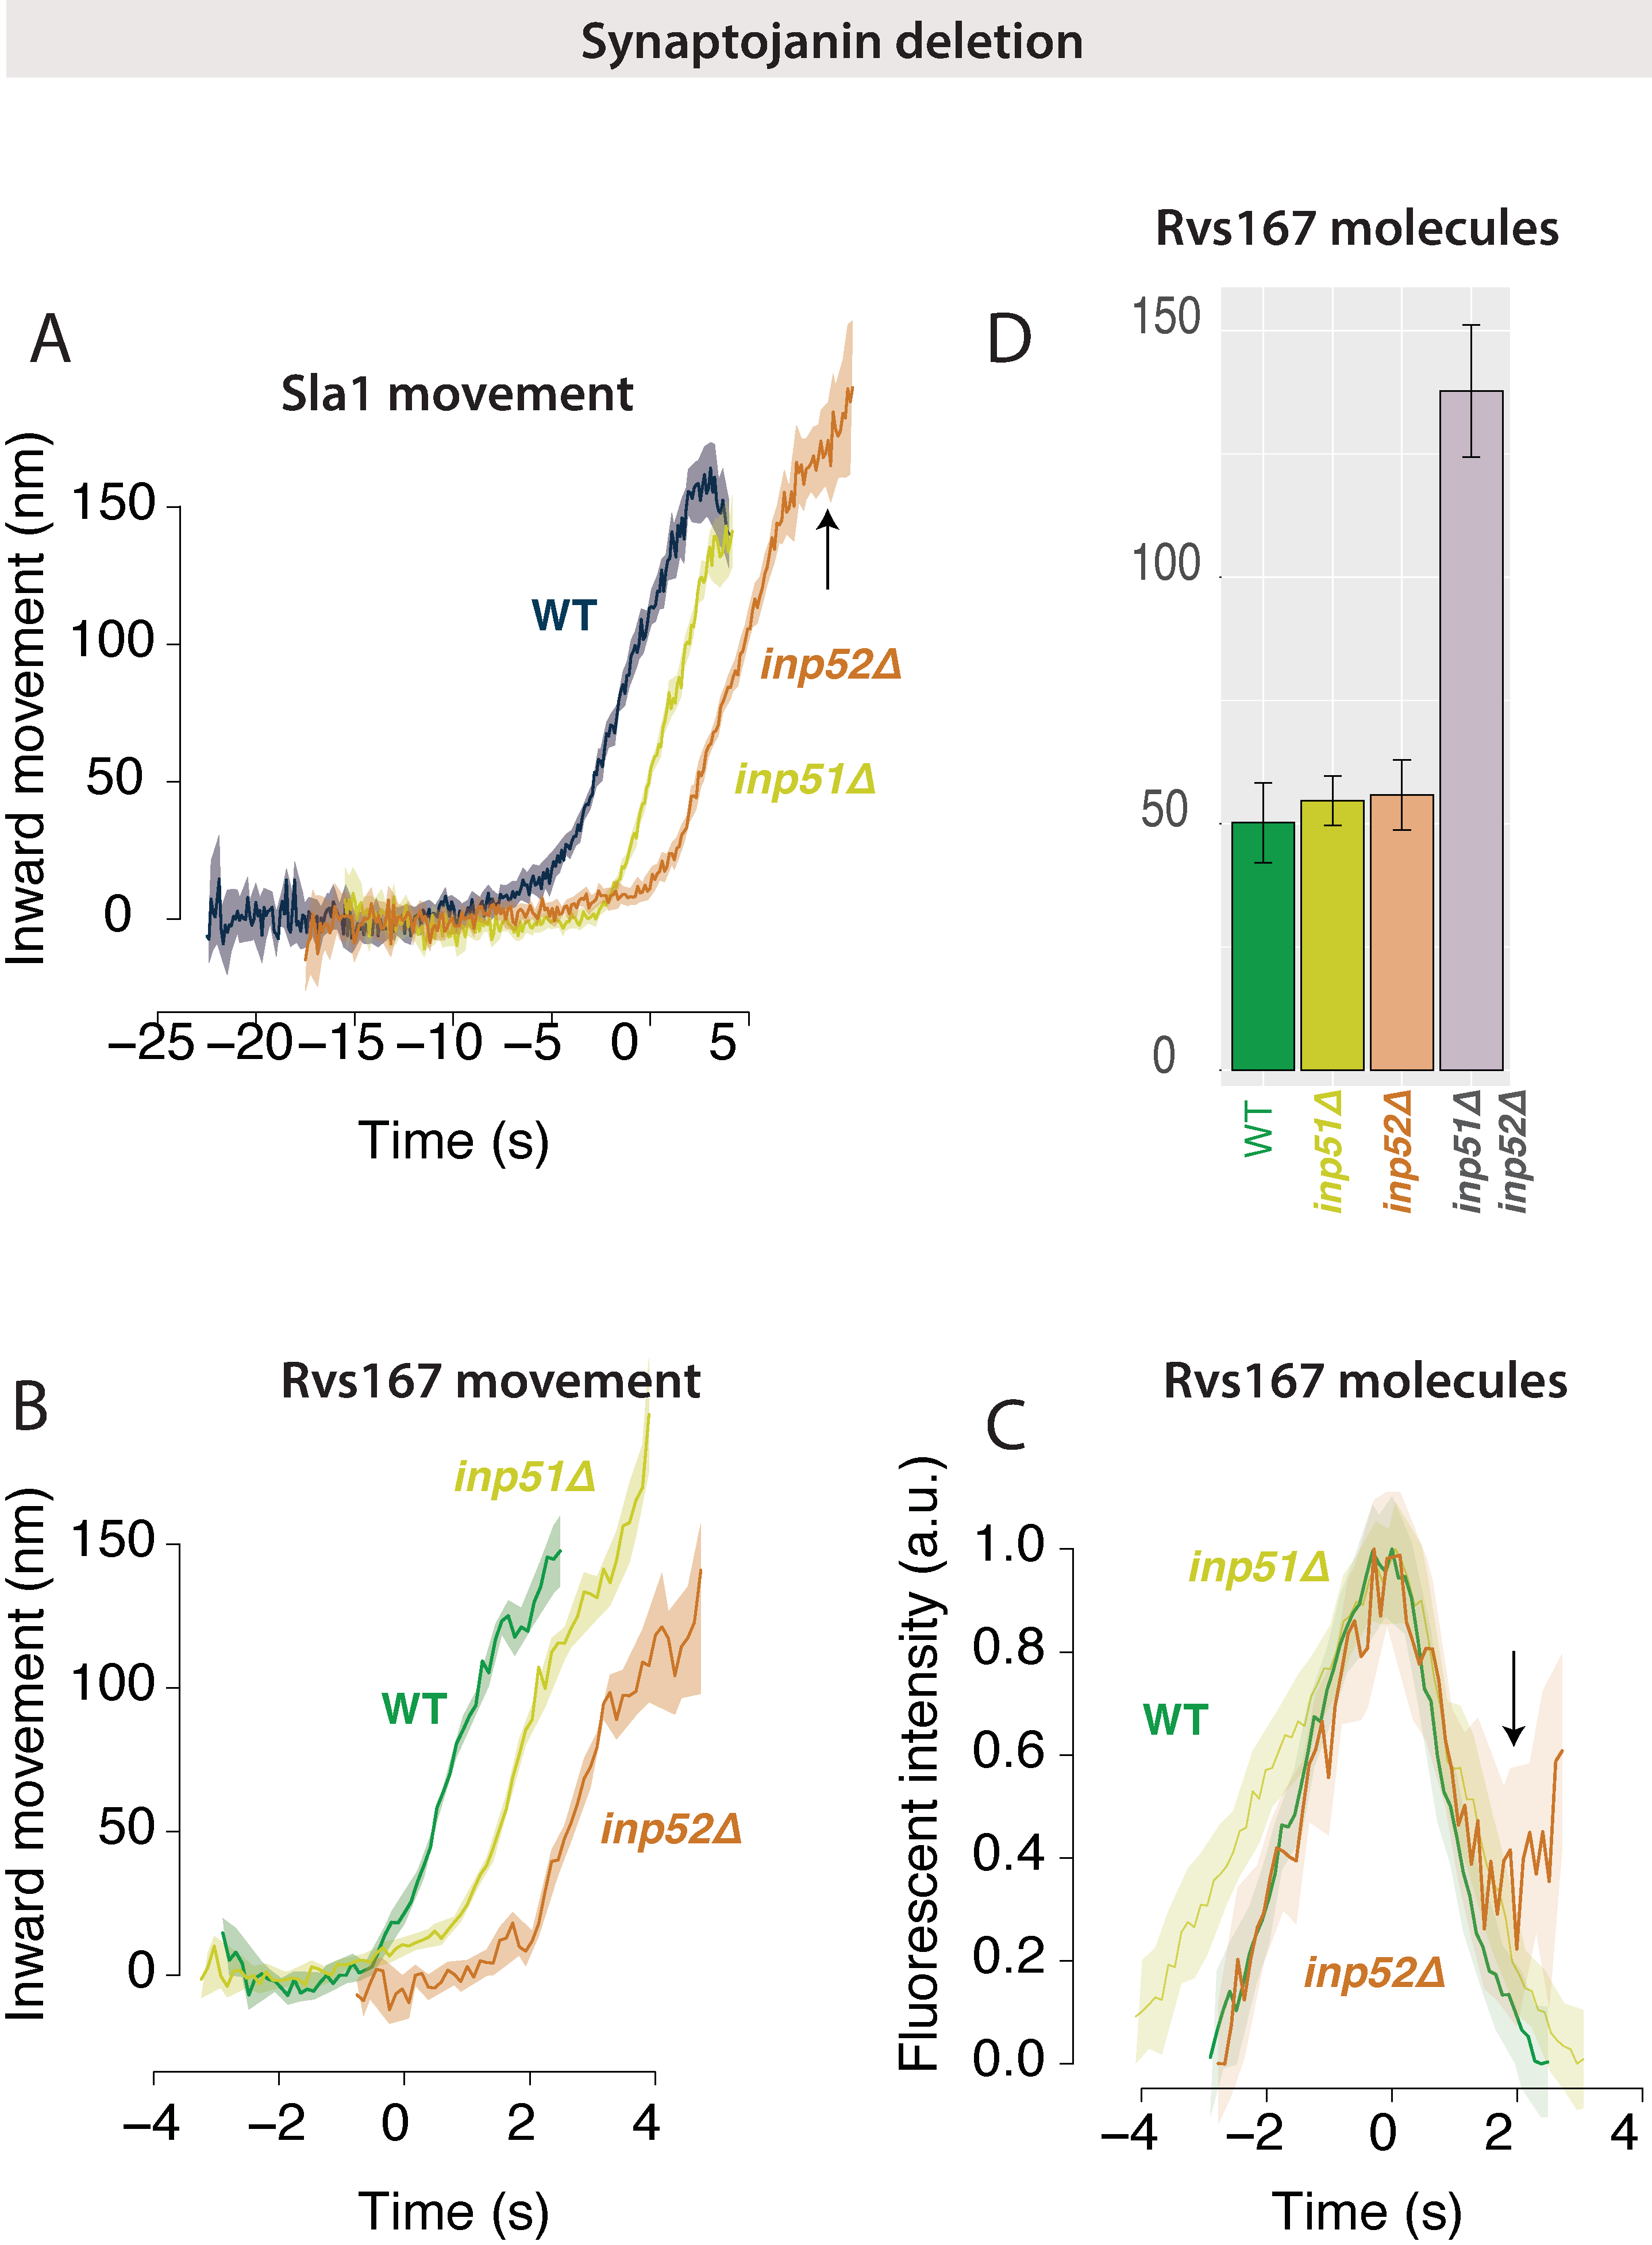
\includegraphics[width=17cm,height=17cm,keepaspectratio]{../../../figures/results_final/inp_movement}
	\caption{Sla1 and Rvs167 in Synaptojanin deletion \label{fig5}}
	\end{figure}
	
	\subsection{Protein friction does not induce membrane scission }
		Yeast dynamin is the obvious solution to membrane scission. Although none of the three dynamin- like proteins has a proline-rich domain, one of the yeast dynamins, Vps1 has been suggested to be involved in endocytosis11,12. Rooij et al., suggest that Vps1 localizes to endocytic sites in the late scission stage, and that the vps1Δ rvs167Δ double mutant increases membrane retraction rates after invagination, an indication of scission failure. Vps1-GFP does not localize to endocytic sites in Gadila et at.,13, but localizes to the golgi body and to vacuoles. Kishimoto et al, do not find a colocalization between Vps1 and Abp1 localization, and also report that the vps1Δ rvs167Δ  double mutation does not affect membrane retraction rates. Vps1 tagged with both GFP as well as superfolded GFP, and imaged by TIRF microscopy fails to colocalize with Abp1 (data not shown, personal communication with Andrea Picco). The debate concerning the involvement of Vps1 in membrane scission in yeast has been compounded by the possibility that the GFP tag at the Vps1 C-terminal could interfere with its localization to endocytic sites, or its interaction with the Rvs complex. 
			Yeast dynamin is the obvious solution to membrane scission. Although none of the three dynamin- like proteins has a proline-rich domain, one of the yeast dynamins, Vps1 has been suggested to be involved in endocytosis11,12. Rooij et al., suggest that Vps1 localizes to endocytic sites in the late scission stage, and that the vps1Δ rvs167Δ double mutant increases membrane retraction rates after invagination, an indication of scission failure. Vps1-GFP does not localize to endocytic sites in Gadila et at.,13, but localizes to the golgi body and to vacuoles. Kishimoto et al, do not find a colocalization between Vps1 and Abp1 localization, and also report that the vps1Δ rvs167Δ  double mutation does not affect membrane retraction rates. Vps1 tagged with both GFP as well as superfolded GFP, and imaged by TIRF microscopy fails to colocalize with Abp1 (data not shown, personal communication with Andrea Picco). The debate concerning the involvement of Vps1 in membrane scission in yeast has been compounded by the possibility that the GFP tag at the Vps1 C-terminal could interfere with its localization to endocytic sites, or its interaction with the Rvs complex. 
	
	\subsection{Scission timing is determined by actin forces, \\
		BAR domains prevent scission}